% Options for packages loaded elsewhere
\PassOptionsToPackage{unicode}{hyperref}
\PassOptionsToPackage{hyphens}{url}
%
\documentclass[
]{article}
\usepackage{amsmath,amssymb}
\usepackage{lmodern}
\usepackage{ifxetex,ifluatex}
\ifnum 0\ifxetex 1\fi\ifluatex 1\fi=0 % if pdftex
  \usepackage[T1]{fontenc}
  \usepackage[utf8]{inputenc}
  \usepackage{textcomp} % provide euro and other symbols
\else % if luatex or xetex
  \usepackage{unicode-math}
  \defaultfontfeatures{Scale=MatchLowercase}
  \defaultfontfeatures[\rmfamily]{Ligatures=TeX,Scale=1}
\fi
% Use upquote if available, for straight quotes in verbatim environments
\IfFileExists{upquote.sty}{\usepackage{upquote}}{}
\IfFileExists{microtype.sty}{% use microtype if available
  \usepackage[]{microtype}
  \UseMicrotypeSet[protrusion]{basicmath} % disable protrusion for tt fonts
}{}
\makeatletter
\@ifundefined{KOMAClassName}{% if non-KOMA class
  \IfFileExists{parskip.sty}{%
    \usepackage{parskip}
  }{% else
    \setlength{\parindent}{0pt}
    \setlength{\parskip}{6pt plus 2pt minus 1pt}}
}{% if KOMA class
  \KOMAoptions{parskip=half}}
\makeatother
\usepackage{xcolor}
\IfFileExists{xurl.sty}{\usepackage{xurl}}{} % add URL line breaks if available
\IfFileExists{bookmark.sty}{\usepackage{bookmark}}{\usepackage{hyperref}}
\hypersetup{
  pdftitle={Leaf-light-project},
  pdfauthor={cong},
  hidelinks,
  pdfcreator={LaTeX via pandoc}}
\urlstyle{same} % disable monospaced font for URLs
\usepackage[margin=1in]{geometry}
\usepackage{color}
\usepackage{fancyvrb}
\newcommand{\VerbBar}{|}
\newcommand{\VERB}{\Verb[commandchars=\\\{\}]}
\DefineVerbatimEnvironment{Highlighting}{Verbatim}{commandchars=\\\{\}}
% Add ',fontsize=\small' for more characters per line
\usepackage{framed}
\definecolor{shadecolor}{RGB}{248,248,248}
\newenvironment{Shaded}{\begin{snugshade}}{\end{snugshade}}
\newcommand{\AlertTok}[1]{\textcolor[rgb]{0.94,0.16,0.16}{#1}}
\newcommand{\AnnotationTok}[1]{\textcolor[rgb]{0.56,0.35,0.01}{\textbf{\textit{#1}}}}
\newcommand{\AttributeTok}[1]{\textcolor[rgb]{0.77,0.63,0.00}{#1}}
\newcommand{\BaseNTok}[1]{\textcolor[rgb]{0.00,0.00,0.81}{#1}}
\newcommand{\BuiltInTok}[1]{#1}
\newcommand{\CharTok}[1]{\textcolor[rgb]{0.31,0.60,0.02}{#1}}
\newcommand{\CommentTok}[1]{\textcolor[rgb]{0.56,0.35,0.01}{\textit{#1}}}
\newcommand{\CommentVarTok}[1]{\textcolor[rgb]{0.56,0.35,0.01}{\textbf{\textit{#1}}}}
\newcommand{\ConstantTok}[1]{\textcolor[rgb]{0.00,0.00,0.00}{#1}}
\newcommand{\ControlFlowTok}[1]{\textcolor[rgb]{0.13,0.29,0.53}{\textbf{#1}}}
\newcommand{\DataTypeTok}[1]{\textcolor[rgb]{0.13,0.29,0.53}{#1}}
\newcommand{\DecValTok}[1]{\textcolor[rgb]{0.00,0.00,0.81}{#1}}
\newcommand{\DocumentationTok}[1]{\textcolor[rgb]{0.56,0.35,0.01}{\textbf{\textit{#1}}}}
\newcommand{\ErrorTok}[1]{\textcolor[rgb]{0.64,0.00,0.00}{\textbf{#1}}}
\newcommand{\ExtensionTok}[1]{#1}
\newcommand{\FloatTok}[1]{\textcolor[rgb]{0.00,0.00,0.81}{#1}}
\newcommand{\FunctionTok}[1]{\textcolor[rgb]{0.00,0.00,0.00}{#1}}
\newcommand{\ImportTok}[1]{#1}
\newcommand{\InformationTok}[1]{\textcolor[rgb]{0.56,0.35,0.01}{\textbf{\textit{#1}}}}
\newcommand{\KeywordTok}[1]{\textcolor[rgb]{0.13,0.29,0.53}{\textbf{#1}}}
\newcommand{\NormalTok}[1]{#1}
\newcommand{\OperatorTok}[1]{\textcolor[rgb]{0.81,0.36,0.00}{\textbf{#1}}}
\newcommand{\OtherTok}[1]{\textcolor[rgb]{0.56,0.35,0.01}{#1}}
\newcommand{\PreprocessorTok}[1]{\textcolor[rgb]{0.56,0.35,0.01}{\textit{#1}}}
\newcommand{\RegionMarkerTok}[1]{#1}
\newcommand{\SpecialCharTok}[1]{\textcolor[rgb]{0.00,0.00,0.00}{#1}}
\newcommand{\SpecialStringTok}[1]{\textcolor[rgb]{0.31,0.60,0.02}{#1}}
\newcommand{\StringTok}[1]{\textcolor[rgb]{0.31,0.60,0.02}{#1}}
\newcommand{\VariableTok}[1]{\textcolor[rgb]{0.00,0.00,0.00}{#1}}
\newcommand{\VerbatimStringTok}[1]{\textcolor[rgb]{0.31,0.60,0.02}{#1}}
\newcommand{\WarningTok}[1]{\textcolor[rgb]{0.56,0.35,0.01}{\textbf{\textit{#1}}}}
\usepackage{graphicx}
\makeatletter
\def\maxwidth{\ifdim\Gin@nat@width>\linewidth\linewidth\else\Gin@nat@width\fi}
\def\maxheight{\ifdim\Gin@nat@height>\textheight\textheight\else\Gin@nat@height\fi}
\makeatother
% Scale images if necessary, so that they will not overflow the page
% margins by default, and it is still possible to overwrite the defaults
% using explicit options in \includegraphics[width, height, ...]{}
\setkeys{Gin}{width=\maxwidth,height=\maxheight,keepaspectratio}
% Set default figure placement to htbp
\makeatletter
\def\fps@figure{htbp}
\makeatother
\setlength{\emergencystretch}{3em} % prevent overfull lines
\providecommand{\tightlist}{%
  \setlength{\itemsep}{0pt}\setlength{\parskip}{0pt}}
\setcounter{secnumdepth}{-\maxdimen} % remove section numbering
\usepackage{booktabs}
\usepackage{longtable}
\usepackage{array}
\usepackage{multirow}
\usepackage{wrapfig}
\usepackage{float}
\usepackage{colortbl}
\usepackage{pdflscape}
\usepackage{tabu}
\usepackage{threeparttable}
\usepackage{threeparttablex}
\usepackage[normalem]{ulem}
\usepackage{makecell}
\usepackage{xcolor}
\ifluatex
  \usepackage{selnolig}  % disable illegal ligatures
\fi

\title{Leaf-light-project}
\author{cong}
\date{2021/12/23}

\begin{document}
\maketitle

{
\setcounter{tocdepth}{2}
\tableofcontents
}
\hypertarget{background}{%
\section{Background}\label{background}}

The big light project puts a LED light into old-growth, secondary and
man made forest(rubber tree forest) separetely, which shines at night.
We rekon it as a long term disturbance to forest which has continued
more than one year. Now we want to know whether this disturbance would
effect the understory or not.

\hypertarget{our-hypothesis}{%
\subsection{Our hypothesis}\label{our-hypothesis}}

\begin{enumerate}
\def\labelenumi{\arabic{enumi})}
\tightlist
\item
  Prolong the light time may effect the nutrition circulation of
  understory
\item
  LED light attracts insects and insects dead may increase soil
  nitrogen, then effect the nutrition circulation of understory.
\end{enumerate}

\hypertarget{place-and-species-i-choosed}{%
\subsection{Place and species I
choosed}\label{place-and-species-i-choosed}}

We choose man made forest, for simulating the street tree and species
Colocasia\_gigantea and Melastoma\_candidum

\hypertarget{method}{%
\subsection{method}\label{method}}

we punch leaf using leaf-disc to measure leaf nutrition.

\hypertarget{data-exploration}{%
\section{Data Exploration}\label{data-exploration}}

the pacakges we'll use:

\begin{Shaded}
\begin{Highlighting}[]
\FunctionTok{library}\NormalTok{(kableExtra)}
\FunctionTok{library}\NormalTok{(tidyverse)}
\CommentTok{\#\textgreater{} {-}{-} Attaching packages {-}{-}{-}{-}{-}{-}{-}{-}{-}{-}{-}{-}{-}{-}{-}{-}{-}{-}{-}{-}{-}{-}{-}{-}{-}{-}{-}{-}{-}{-}{-}{-}{-}{-}{-}{-}{-}{-}{-} tidyverse 1.3.1 {-}{-}}
\CommentTok{\#\textgreater{} v ggplot2 3.3.5     v purrr   0.3.4}
\CommentTok{\#\textgreater{} v tibble  3.1.6     v dplyr   1.0.7}
\CommentTok{\#\textgreater{} v tidyr   1.1.4     v stringr 1.4.0}
\CommentTok{\#\textgreater{} v readr   2.1.0     v forcats 0.5.1}
\CommentTok{\#\textgreater{} {-}{-} Conflicts {-}{-}{-}{-}{-}{-}{-}{-}{-}{-}{-}{-}{-}{-}{-}{-}{-}{-}{-}{-}{-}{-}{-}{-}{-}{-}{-}{-}{-}{-}{-}{-}{-}{-}{-}{-}{-}{-}{-}{-}{-}{-} tidyverse\_conflicts() {-}{-}}
\CommentTok{\#\textgreater{} x dplyr::filter()     masks stats::filter()}
\CommentTok{\#\textgreater{} x dplyr::group\_rows() masks kableExtra::group\_rows()}
\CommentTok{\#\textgreater{} x dplyr::lag()        masks stats::lag()}
\FunctionTok{library}\NormalTok{(lme4)}
\CommentTok{\#\textgreater{} 载入需要的程辑包:Matrix}
\CommentTok{\#\textgreater{} }
\CommentTok{\#\textgreater{} 载入程辑包:\textquotesingle{}Matrix\textquotesingle{}}
\CommentTok{\#\textgreater{} The following objects are masked from \textquotesingle{}package:tidyr\textquotesingle{}:}
\CommentTok{\#\textgreater{} }
\CommentTok{\#\textgreater{}     expand, pack, unpack}
\end{Highlighting}
\end{Shaded}

input our data

\begin{Shaded}
\begin{Highlighting}[]
\NormalTok{llp }\OtherTok{\textless{}{-}} \FunctionTok{read\_csv}\NormalTok{(}\StringTok{"../data{-}raw/leaf\_light\_project.csv"}\NormalTok{)}
\CommentTok{\#\textgreater{} Rows: 260 Columns: 11}
\CommentTok{\#\textgreater{} {-}{-} Column specification {-}{-}{-}{-}{-}{-}{-}{-}{-}{-}{-}{-}{-}{-}{-}{-}{-}{-}{-}{-}{-}{-}{-}{-}{-}{-}{-}{-}{-}{-}{-}{-}{-}{-}{-}{-}{-}{-}{-}{-}{-}{-}{-}{-}{-}{-}{-}{-}{-}{-}{-}{-}{-}{-}{-}{-}}
\CommentTok{\#\textgreater{} Delimiter: ","}
\CommentTok{\#\textgreater{} chr  (1): species}
\CommentTok{\#\textgreater{} dbl (10): Plot, Distance, angel, individual, leaf ID, disc, disc\_area, fresh...}
\CommentTok{\#\textgreater{} }
\CommentTok{\#\textgreater{} i Use \textasciigrave{}spec()\textasciigrave{} to retrieve the full column specification for this data.}
\CommentTok{\#\textgreater{} i Specify the column types or set \textasciigrave{}show\_col\_types = FALSE\textasciigrave{} to quiet this message.}
\NormalTok{llp[}\DecValTok{1}\SpecialCharTok{:}\DecValTok{5}\NormalTok{,] }\SpecialCharTok{\%\textgreater{}\%} \FunctionTok{kbl}\NormalTok{() }\SpecialCharTok{\%\textgreater{}\%} \FunctionTok{kable\_styling}\NormalTok{()}
\end{Highlighting}
\end{Shaded}

\begin{table}
\centering
\begin{tabular}[t]{r|l|r|r|r|r|r|r|r|r|r}
\hline
Plot & species & Distance & angel & individual & leaf ID & disc & disc\_area & fresh\_weight & dry\_weight & canopy\_openness\\
\hline
5 & Melastoma\_candidum & 7.3 & 246 & 1 & 1 & 5 & 10 & 0.0469 & 0.0133 & 0.093571\\
\hline
5 & Melastoma\_candidum & 7.3 & 246 & 1 & 2 & 5 & 10 & 0.0497 & 0.0140 & 0.093571\\
\hline
5 & Melastoma\_candidum & 7.3 & 246 & 1 & 3 & 5 & 10 & 0.0476 & 0.0141 & 0.093571\\
\hline
5 & Melastoma\_candidum & 7.3 & 246 & 1 & 4 & 5 & 10 & 0.0453 & 0.0140 & 0.093571\\
\hline
5 & Melastoma\_candidum & 7.3 & 246 & 1 & 5 & 5 & 10 & 0.0489 & 0.0158 & 0.093571\\
\hline
\end{tabular}
\end{table}

Then we calculate LMA and show our samples location away from the light.

\begin{Shaded}
\begin{Highlighting}[]
\NormalTok{llp1 }\OtherTok{\textless{}{-}}\NormalTok{ llp }\SpecialCharTok{|}\ErrorTok{\textgreater{}}\FunctionTok{mutate}\NormalTok{(}\AttributeTok{LMA =}\NormalTok{ dry\_weight}\SpecialCharTok{/}\NormalTok{(disc}\SpecialCharTok{*}\NormalTok{pi}\SpecialCharTok{*}\NormalTok{(}\FloatTok{0.005}\NormalTok{)}\SpecialCharTok{\^{}}\DecValTok{2}\NormalTok{))}
\NormalTok{llp1 }\SpecialCharTok{|}\ErrorTok{\textgreater{}} 
  \FunctionTok{mutate}\NormalTok{(}\AttributeTok{x\_loc =}\NormalTok{ Distance}\SpecialCharTok{*}\FunctionTok{cos}\NormalTok{(angel}\SpecialCharTok{*}\NormalTok{pi}\SpecialCharTok{/}\DecValTok{180}\NormalTok{))}\SpecialCharTok{|}\ErrorTok{\textgreater{}}
  \FunctionTok{mutate}\NormalTok{(}\AttributeTok{y\_loc =}\NormalTok{ Distance}\SpecialCharTok{*}\FunctionTok{sin}\NormalTok{(angel}\SpecialCharTok{*}\NormalTok{pi}\SpecialCharTok{/}\DecValTok{180}\NormalTok{))}\SpecialCharTok{|}\ErrorTok{\textgreater{}}
  \FunctionTok{ggplot}\NormalTok{(}\FunctionTok{aes}\NormalTok{(x\_loc, y\_loc, }\AttributeTok{size =}\NormalTok{ LMA))}\SpecialCharTok{+}
  \FunctionTok{geom\_point}\NormalTok{(}\AttributeTok{shape =}\DecValTok{17}\NormalTok{)}\SpecialCharTok{+}
  \FunctionTok{facet\_grid}\NormalTok{(}\AttributeTok{cols =} \FunctionTok{vars}\NormalTok{(species))}\SpecialCharTok{+}
  \FunctionTok{theme\_bw}\NormalTok{()}
\end{Highlighting}
\end{Shaded}

\begin{center}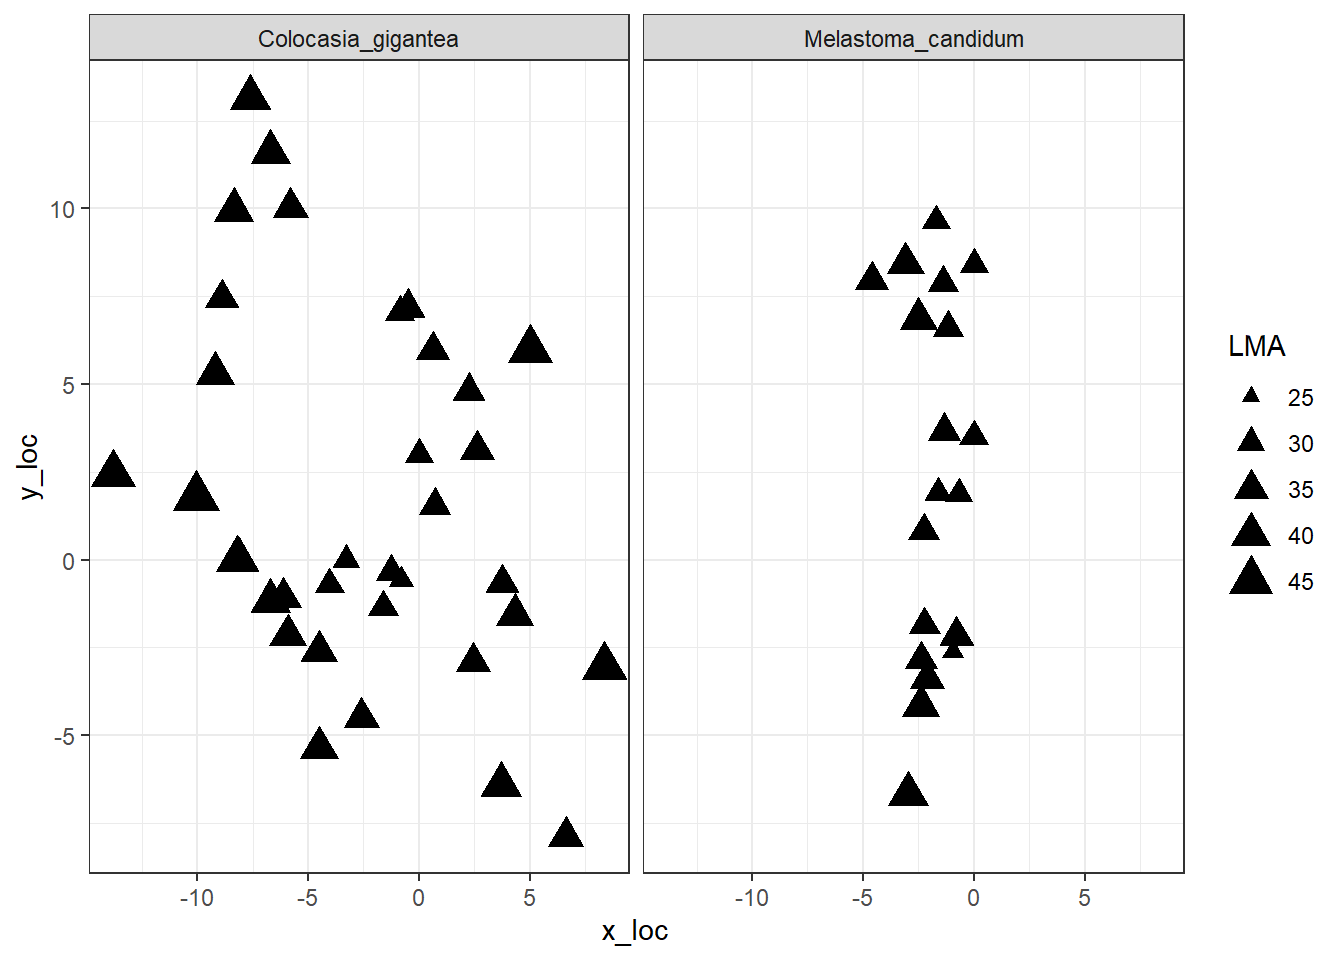
\includegraphics{leaf_light_project_showing_files/figure-latex/unnamed-chunk-3-1} \end{center}

(Notation: coordinate (0,0) is where the light is.)

Next, because we want to know whether light give an effect to
understory, so we consider a graph between LMA and Distance away from
the light which is on behalf of the gradient of light strength.

\begin{Shaded}
\begin{Highlighting}[]
\NormalTok{llp1 }\SpecialCharTok{|}\ErrorTok{\textgreater{}} 
  \FunctionTok{filter}\NormalTok{(Plot }\SpecialCharTok{==} \DecValTok{2}\NormalTok{) }\SpecialCharTok{|}\ErrorTok{\textgreater{}}
\FunctionTok{ggplot}\NormalTok{(}\FunctionTok{aes}\NormalTok{(}\AttributeTok{x =}\NormalTok{ Distance, }\AttributeTok{y =}\NormalTok{ LMA))}\SpecialCharTok{+}
  \FunctionTok{geom\_point}\NormalTok{()}\SpecialCharTok{+}
  \FunctionTok{labs}\NormalTok{(}\AttributeTok{title =} \StringTok{"LMA\_Colocasia\_gigantea"}\NormalTok{)}\SpecialCharTok{+}
  \FunctionTok{theme\_bw}\NormalTok{()}
\end{Highlighting}
\end{Shaded}

\begin{center}\includegraphics{leaf_light_project_showing_files/figure-latex/unnamed-chunk-4-1} \end{center}

\begin{Shaded}
\begin{Highlighting}[]
\NormalTok{llp1 }\SpecialCharTok{|}\ErrorTok{\textgreater{}}
  \FunctionTok{filter}\NormalTok{(Plot }\SpecialCharTok{==} \DecValTok{5}\NormalTok{) }\SpecialCharTok{|}\ErrorTok{\textgreater{}}
\FunctionTok{ggplot}\NormalTok{(}\FunctionTok{aes}\NormalTok{(}\AttributeTok{x =}\NormalTok{ Distance, }\AttributeTok{y =}\NormalTok{ LMA))}\SpecialCharTok{+}
  \FunctionTok{geom\_point}\NormalTok{()}\SpecialCharTok{+}
   \FunctionTok{labs}\NormalTok{(}\AttributeTok{title =} \StringTok{"LMA\_Melastoma\_candidum"}\NormalTok{)}\SpecialCharTok{+}
  \FunctionTok{theme\_bw}\NormalTok{()}
\end{Highlighting}
\end{Shaded}

\begin{center}\includegraphics{leaf_light_project_showing_files/figure-latex/unnamed-chunk-5-1} \end{center}

(We see there can be a negative correlation between LMA and Distance,
while we can't simply draw the conclusion based on that, instead we add
canopy openness into our consideration. )

\begin{Shaded}
\begin{Highlighting}[]
\NormalTok{llp1}\SpecialCharTok{|}\ErrorTok{\textgreater{}} 
  \FunctionTok{ggplot}\NormalTok{(}\FunctionTok{aes}\NormalTok{(}\AttributeTok{x =}\NormalTok{ LMA))}\SpecialCharTok{+}
  \FunctionTok{facet\_grid}\NormalTok{(}\AttributeTok{cols =} \FunctionTok{vars}\NormalTok{(species))}\SpecialCharTok{+}
  \FunctionTok{geom\_histogram}\NormalTok{()}
\CommentTok{\#\textgreater{} \textasciigrave{}stat\_bin()\textasciigrave{} using \textasciigrave{}bins = 30\textasciigrave{}. Pick better value with \textasciigrave{}binwidth\textasciigrave{}.}
\end{Highlighting}
\end{Shaded}

\begin{center}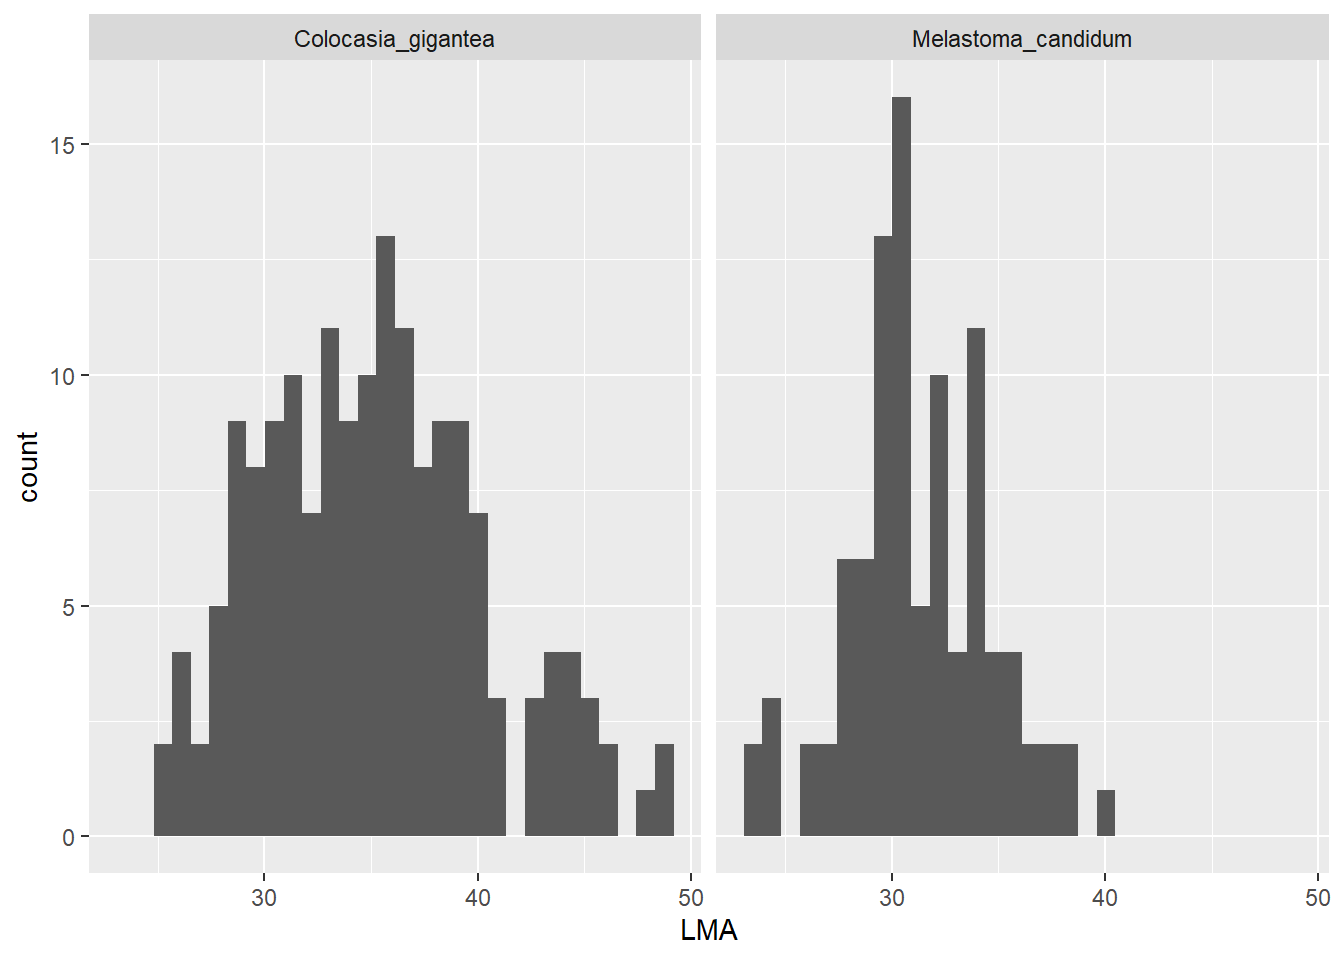
\includegraphics{leaf_light_project_showing_files/figure-latex/unnamed-chunk-6-1} \end{center}

\hypertarget{data-mining}{%
\section{Data Mining}\label{data-mining}}

\begin{Shaded}
\begin{Highlighting}[]
\NormalTok{mod }\OtherTok{\textless{}{-}} \FunctionTok{lmer}\NormalTok{(}\AttributeTok{data =}\NormalTok{ llp1, }\AttributeTok{formula =}\NormalTok{ LMA }\SpecialCharTok{\textasciitilde{}} \FunctionTok{log}\NormalTok{(Distance)}\SpecialCharTok{*}\FunctionTok{log}\NormalTok{(canopy\_openness)}\SpecialCharTok{+}\NormalTok{(}\DecValTok{1}\SpecialCharTok{|}\NormalTok{species))}
\FunctionTok{summary}\NormalTok{(mod)}
\CommentTok{\#\textgreater{} Linear mixed model fit by REML [\textquotesingle{}lmerMod\textquotesingle{}]}
\CommentTok{\#\textgreater{} Formula: LMA \textasciitilde{} log(Distance) * log(canopy\_openness) + (1 | species)}
\CommentTok{\#\textgreater{}    Data: llp1}
\CommentTok{\#\textgreater{} }
\CommentTok{\#\textgreater{} REML criterion at convergence: 1394.3}
\CommentTok{\#\textgreater{} }
\CommentTok{\#\textgreater{} Scaled residuals: }
\CommentTok{\#\textgreater{}      Min       1Q   Median       3Q      Max }
\CommentTok{\#\textgreater{} {-}2.75665 {-}0.75270  0.02021  0.62920  3.00758 }
\CommentTok{\#\textgreater{} }
\CommentTok{\#\textgreater{} Random effects:}
\CommentTok{\#\textgreater{}  Groups   Name        Variance Std.Dev.}
\CommentTok{\#\textgreater{}  species  (Intercept)  4.657   2.158   }
\CommentTok{\#\textgreater{}  Residual             12.554   3.543   }
\CommentTok{\#\textgreater{} Number of obs: 260, groups:  species, 2}
\CommentTok{\#\textgreater{} }
\CommentTok{\#\textgreater{} Fixed effects:}
\CommentTok{\#\textgreater{}                                    Estimate Std. Error t value}
\CommentTok{\#\textgreater{} (Intercept)                          22.714      4.139   5.487}
\CommentTok{\#\textgreater{} log(Distance)                        11.460      2.393   4.789}
\CommentTok{\#\textgreater{} log(canopy\_openness)                 {-}1.392      1.713  {-}0.812}
\CommentTok{\#\textgreater{} log(Distance):log(canopy\_openness)    2.836      1.039   2.731}
\CommentTok{\#\textgreater{} }
\CommentTok{\#\textgreater{} Correlation of Fixed Effects:}
\CommentTok{\#\textgreater{}             (Intr) lg(Ds) lg(c\_)}
\CommentTok{\#\textgreater{} log(Distnc) {-}0.869              }
\CommentTok{\#\textgreater{} lg(cnpy\_pn)  0.916 {-}0.924       }
\CommentTok{\#\textgreater{} lg(Dst):(\_) {-}0.870  0.987 {-}0.950}
\end{Highlighting}
\end{Shaded}

\hypertarget{stan}{%
\section{stan}\label{stan}}

\hypertarget{example}{%
\subsection{example}\label{example}}

\begin{Shaded}
\begin{Highlighting}[]
\FunctionTok{library}\NormalTok{(rstan)}
\FunctionTok{library}\NormalTok{(bayesplot)}
\NormalTok{rstan}\SpecialCharTok{::}\FunctionTok{rstan\_options}\NormalTok{(}\AttributeTok{auto\_write =} \ConstantTok{TRUE}\NormalTok{)}
\FunctionTok{options}\NormalTok{(}\AttributeTok{mc.cores =}\NormalTok{ parallel}\SpecialCharTok{::}\FunctionTok{detectCores}\NormalTok{()) }\CommentTok{\# Run on multiple cores}
\end{Highlighting}
\end{Shaded}

Data for Melastoma\_candidum

\begin{Shaded}
\begin{Highlighting}[]
\NormalTok{sp1 }\OtherTok{\textless{}{-}}\NormalTok{ llp1 }\SpecialCharTok{|}\ErrorTok{\textgreater{}}
  \FunctionTok{filter}\NormalTok{(species }\SpecialCharTok{==} \StringTok{"Melastoma\_candidum"}\NormalTok{)}

\NormalTok{x }\OtherTok{\textless{}{-}} \FunctionTok{cbind}\NormalTok{(}\DecValTok{1}\NormalTok{,}
            \FunctionTok{log}\NormalTok{(}\DecValTok{1}\SpecialCharTok{/}\NormalTok{(sp1}\SpecialCharTok{$}\NormalTok{Distance)}\SpecialCharTok{\^{}}\DecValTok{2}\NormalTok{) }\SpecialCharTok{|}\ErrorTok{\textgreater{}} \FunctionTok{scale}\NormalTok{(),}
            \FunctionTok{scale}\NormalTok{(sp1}\SpecialCharTok{$}\NormalTok{canopy\_openness))}

\NormalTok{x }\OtherTok{\textless{}{-}} \FunctionTok{cbind}\NormalTok{(x, x[,}\DecValTok{2}\NormalTok{] }\SpecialCharTok{*}\NormalTok{ x[,}\DecValTok{3}\NormalTok{])}

\NormalTok{list\_d }\OtherTok{\textless{}{-}} \FunctionTok{list}\NormalTok{(}
  \AttributeTok{N =} \FunctionTok{nrow}\NormalTok{(sp1),}
  \AttributeTok{J =}\NormalTok{ sp1}\SpecialCharTok{$}\NormalTok{individual }\SpecialCharTok{|}\ErrorTok{\textgreater{}} \FunctionTok{unique}\NormalTok{() }\SpecialCharTok{|}\ErrorTok{\textgreater{}} \FunctionTok{length}\NormalTok{(),}
  \AttributeTok{K =} \DecValTok{4}\NormalTok{,}
  \AttributeTok{ind =}\NormalTok{ sp1}\SpecialCharTok{$}\NormalTok{individual,}
  \AttributeTok{x =}\NormalTok{ x,}
  \AttributeTok{y =} \FunctionTok{log}\NormalTok{(sp1}\SpecialCharTok{$}\NormalTok{LMA))}
\end{Highlighting}
\end{Shaded}

\hypertarget{mathematical-model}{%
\paragraph*{Mathematical model}\label{mathematical-model}}
\addcontentsline{toc}{paragraph}{Mathematical model}

Main likelihood functions: \[
y_{i,j} \sim \mathcal{N}(\mu_{i,j}, \sigma)  \\
\mu_{i,j} = \boldsymbol{X} \cdot \boldsymbol{\beta} + \phi_j\\
\phi_j \sim \mathcal{N}(0, \tau)
\]

where,

\begin{itemize}
\item
  \(y_{i,j}\) is log(LMA) of leaf disc \emph{i} of individual \emph{j},
\item
  \(\sigma\) is the standard deviation of the model,
\item
  \(\boldsymbol{X}\) is an \(n \times 4\) matrix with intercepts,
  distance, canopy\_openness and the interaction between distance and
  canopy\_openness,
\item
  \(\boldsymbol{\beta}\) is a coefficient vector of size 4 (intercepts,
  distance, canopy\_openness and the interaction between distance and
  canopy\_openness),
\item
  \(\phi_j\) is the vayring intercept for individuals,
\item
  \(\tau\) is the scaling parameter for individual effects
\end{itemize}

Prior:

\begin{itemize}
\tightlist
\item
  we usually use weakly informative priors and we don't use
  non-informative prirors such as unif(0, 1000).
\end{itemize}

\[
\boldsymbol{\beta} \sim \mathcal{N}(0, 5) \\
\]

Hyperprior:

\begin{itemize}
\tightlist
\item
  Half-cauchy works best for the scaling parameters for varying
  intercepts
\end{itemize}

\[
\boldsymbol{\tau} \sim \text{Half-Caucy}(0, 2.5) \\
\]

In reality, we use a lot of tricks to make the above model works better.
For example, we do not try to fit the individual effects directly, but
instead, we fit a latent Gaussian variable from which we can recover the
individual effects.

\[
\phi_j  \sim \mathcal{N}(0, \tau)
\]

cab be rewritten as:

\[
\phi_j =  \tau \cdot \tilde{\phi_j} \\
\tilde{\phi_j} \sim \mathcal{N}(0, 1) \\
\tau \sim \text{Half-cauchy}(0, 2.5)\\
\]

A Half-cauchy distribution can be also represented using the tangent
function and an uniform distribution:

\[
\boldsymbol{\tau} = 2.5 \times tan(\boldsymbol{\tilde{\tau}}) \\
\boldsymbol{\tilde{\tau}} \sim \mathcal{U}(0, \pi / 2)
\]

\begin{Shaded}
\begin{Highlighting}[]
\NormalTok{model }\OtherTok{\textless{}{-}}\NormalTok{ rstan}\SpecialCharTok{::}\FunctionTok{stan\_model}\NormalTok{(}\StringTok{"../stan/model.stan"}\NormalTok{)}
\end{Highlighting}
\end{Shaded}

\begin{Shaded}
\begin{Highlighting}[]
\FunctionTok{writeLines}\NormalTok{(}\FunctionTok{readLines}\NormalTok{(}\StringTok{"../stan/model.stan"}\NormalTok{))}
\end{Highlighting}
\end{Shaded}

\begin{verbatim}
data{
  int<lower=0> N; // number of sample
  int<lower=1> J; // number of individual
  int<lower=1> K; // number of parameters
  matrix[N, K] x; // tree-level predictor
  vector[N] y; //log(LMA)
  int<lower=1,upper=J> ind[N]; // integer
}


parameters{
  matrix[K,1] beta;
  vector[J] phi_raw;
  real<lower=0,upper=pi()/2> tau_unif;
  real<lower=0> sigma;
}

transformed parameters{
  real<lower=0> tau;
  vector[J] phi;
  tau = 2.5 * tan(tau_unif); // implies tau ~ cauchy(0, 2.5)
  phi = phi_raw * tau;
}

model {
  //vector[N] mu;
  //for (n in 1:N) mu[n] = x[n, ] * beta + phi[ind[n]];
  phi_raw ~ std_normal();
  to_vector(beta) ~ normal(0, 5);
  y ~ normal(to_vector(x * beta) + phi[ind], sigma);
}
\end{verbatim}

\begin{Shaded}
\begin{Highlighting}[]
\NormalTok{fit }\OtherTok{\textless{}{-}}\NormalTok{ rstan}\SpecialCharTok{::}\FunctionTok{sampling}\NormalTok{(model,}
            \AttributeTok{data =}\NormalTok{ list\_d,}
            \AttributeTok{verbose =} \ConstantTok{TRUE}\NormalTok{,}
            \AttributeTok{iter =} \DecValTok{2000}\NormalTok{,}
            \AttributeTok{warmup =} \DecValTok{1000}\NormalTok{,}
            \AttributeTok{thin =} \DecValTok{1}\NormalTok{,}
            \AttributeTok{chains =} \DecValTok{4}\NormalTok{,}
            \AttributeTok{refresh =} \DecValTok{200}\NormalTok{,}
            \AttributeTok{seed =} \DecValTok{123}\NormalTok{)}
\CommentTok{\#\textgreater{} }
\CommentTok{\#\textgreater{} CHECKING DATA AND PREPROCESSING FOR MODEL \textquotesingle{}model\textquotesingle{} NOW.}
\CommentTok{\#\textgreater{} }
\CommentTok{\#\textgreater{} COMPILING MODEL \textquotesingle{}model\textquotesingle{} NOW.}
\CommentTok{\#\textgreater{} }
\CommentTok{\#\textgreater{} STARTING SAMPLER FOR MODEL \textquotesingle{}model\textquotesingle{} NOW.}
\end{Highlighting}
\end{Shaded}

\begin{Shaded}
\begin{Highlighting}[]
\FunctionTok{summary}\NormalTok{(fit)}\SpecialCharTok{$}\NormalTok{summary}
\CommentTok{\#\textgreater{}                      mean      se\_mean          sd          2.5\%           25\%}
\CommentTok{\#\textgreater{} beta[1,1]    3.459415e+00 7.853398e{-}04 0.030530273   3.400709374   3.439755005}
\CommentTok{\#\textgreater{} beta[2,1]   {-}4.217701e{-}02 8.895009e{-}04 0.035601825  {-}0.112851838  {-}0.064869256}
\CommentTok{\#\textgreater{} beta[3,1]   {-}6.066213e{-}04 9.227563e{-}04 0.037315900  {-}0.076133762  {-}0.024549484}
\CommentTok{\#\textgreater{} beta[4,1]   {-}3.083868e{-}02 6.313788e{-}04 0.026634990  {-}0.083572593  {-}0.048281005}
\CommentTok{\#\textgreater{} phi\_raw[1]   6.684914e{-}01 1.664479e{-}02 0.713349518  {-}0.756827727   0.191520685}
\CommentTok{\#\textgreater{} phi\_raw[2]   9.094645e{-}01 9.926824e{-}03 0.408960234   0.139765019   0.631546170}
\CommentTok{\#\textgreater{} phi\_raw[3]   4.588917e{-}01 1.601212e{-}02 0.632781780  {-}0.804461566   0.036797751}
\CommentTok{\#\textgreater{} phi\_raw[4]  {-}4.399054e{-}02 7.877831e{-}03 0.374580264  {-}0.780476272  {-}0.302218183}
\CommentTok{\#\textgreater{} phi\_raw[5]   1.169361e{-}01 8.087798e{-}03 0.383490651  {-}0.635332749  {-}0.131444116}
\CommentTok{\#\textgreater{} phi\_raw[6]  {-}1.649391e+00 1.338614e{-}02 0.569026117  {-}2.807049285  {-}2.017514902}
\CommentTok{\#\textgreater{} phi\_raw[7]   1.585166e+00 1.751336e{-}02 0.807104881   0.019132666   1.031307790}
\CommentTok{\#\textgreater{} phi\_raw[8]  {-}6.090502e{-}01 1.182087e{-}02 0.535483923  {-}1.642468384  {-}0.978791784}
\CommentTok{\#\textgreater{} phi\_raw[9]   2.194273e{-}01 1.266569e{-}02 0.522747700  {-}0.832486846  {-}0.128603272}
\CommentTok{\#\textgreater{} phi\_raw[10] {-}4.720144e{-}01 1.015264e{-}02 0.447495288  {-}1.334117775  {-}0.779435176}
\CommentTok{\#\textgreater{} phi\_raw[11] {-}3.662253e{-}01 8.371914e{-}03 0.371679664  {-}1.097309931  {-}0.611605487}
\CommentTok{\#\textgreater{} phi\_raw[12]  3.018512e{-}01 8.517681e{-}03 0.373659135  {-}0.411958781   0.044866642}
\CommentTok{\#\textgreater{} phi\_raw[13] {-}8.965657e{-}01 1.173896e{-}02 0.521534788  {-}1.920424495  {-}1.250224968}
\CommentTok{\#\textgreater{} phi\_raw[14]  7.402119e{-}01 9.727350e{-}03 0.434684793  {-}0.063503648   0.444242291}
\CommentTok{\#\textgreater{} phi\_raw[15] {-}5.413399e{-}01 9.301956e{-}03 0.426498219  {-}1.398656395  {-}0.832494995}
\CommentTok{\#\textgreater{} phi\_raw[16] {-}1.083221e+00 1.032768e{-}02 0.457129601  {-}1.997108614  {-}1.394973818}
\CommentTok{\#\textgreater{} phi\_raw[17]  1.160439e+00 1.391346e{-}02 0.625891867  {-}0.058789727   0.739203055}
\CommentTok{\#\textgreater{} phi\_raw[18]  3.529175e{-}01 9.923761e{-}03 0.469646899  {-}0.565044761   0.027482412}
\CommentTok{\#\textgreater{} phi\_raw[19] {-}8.918375e{-}01 1.301269e{-}02 0.581157935  {-}2.005837678  {-}1.294028332}
\CommentTok{\#\textgreater{} tau\_unif     3.937281e{-}02 2.605414e{-}04 0.008486024   0.026647742   0.033278082}
\CommentTok{\#\textgreater{} sigma        5.429960e{-}02 9.485467e{-}05 0.004509095   0.046222650   0.051225495}
\CommentTok{\#\textgreater{} tau          9.849056e{-}02 6.526393e{-}04 0.021258000   0.066635129   0.083225930}
\CommentTok{\#\textgreater{} phi[1]       6.390834e{-}02 1.647767e{-}03 0.070519058  {-}0.077111914   0.018610719}
\CommentTok{\#\textgreater{} phi[2]       8.667453e{-}02 8.652838e{-}04 0.037621220   0.014971126   0.061600457}
\CommentTok{\#\textgreater{} phi[3]       4.380325e{-}02 1.603377e{-}03 0.062738376  {-}0.080983231   0.003154367}
\CommentTok{\#\textgreater{} phi[4]      {-}3.961511e{-}03 7.816415e{-}04 0.036745247  {-}0.076656433  {-}0.028568320}
\CommentTok{\#\textgreater{} phi[5]       1.117928e{-}02 8.082640e{-}04 0.037745253  {-}0.064328086  {-}0.012582282}
\CommentTok{\#\textgreater{} phi[6]      {-}1.564174e{-}01 9.781927e{-}04 0.048742891  {-}0.254440532  {-}0.187173361}
\CommentTok{\#\textgreater{} phi[7]       1.504259e{-}01 1.637569e{-}03 0.076152419   0.001611483   0.101117362}
\CommentTok{\#\textgreater{} phi[8]      {-}5.776885e{-}02 1.121579e{-}03 0.052518027  {-}0.163906988  {-}0.091411678}
\CommentTok{\#\textgreater{} phi[9]       2.090914e{-}02 1.293484e{-}03 0.052266795  {-}0.083749701  {-}0.012662683}
\CommentTok{\#\textgreater{} phi[10]     {-}4.443222e{-}02 9.716910e{-}04 0.043447038  {-}0.128651018  {-}0.073126835}
\CommentTok{\#\textgreater{} phi[11]     {-}3.442275e{-}02 7.994778e{-}04 0.035715209  {-}0.103112730  {-}0.057971242}
\CommentTok{\#\textgreater{} phi[12]      2.884252e{-}02 8.368405e{-}04 0.036215285  {-}0.039175742   0.004344796}
\CommentTok{\#\textgreater{} phi[13]     {-}8.478522e{-}02 1.074608e{-}03 0.048491380  {-}0.182592574  {-}0.115599688}
\CommentTok{\#\textgreater{} phi[14]      7.045599e{-}02 9.017627e{-}04 0.040977679  {-}0.007031062   0.043150119}
\CommentTok{\#\textgreater{} phi[15]     {-}5.125951e{-}02 8.464533e{-}04 0.040289229  {-}0.131300068  {-}0.077986656}
\CommentTok{\#\textgreater{} phi[16]     {-}1.025267e{-}01 8.231940e{-}04 0.040209865  {-}0.182435842  {-}0.129081090}
\CommentTok{\#\textgreater{} phi[17]      1.100477e{-}01 1.262728e{-}03 0.058846223  {-}0.005532723   0.071863670}
\CommentTok{\#\textgreater{} phi[18]      3.353886e{-}02 9.727631e{-}04 0.045858556  {-}0.056784222   0.002611720}
\CommentTok{\#\textgreater{} phi[19]     {-}8.486760e{-}02 1.217299e{-}03 0.055892865  {-}0.198489046  {-}0.121157580}
\CommentTok{\#\textgreater{} lp\_\_         2.146476e+02 1.592966e{-}01 4.755898672 204.288106361 211.603486874}
\CommentTok{\#\textgreater{}                       50\%          75\%         97.5\%     n\_eff      Rhat}
\CommentTok{\#\textgreater{} beta[1,1]    3.459649e+00   3.47952132   3.518213629 1511.2843 1.0026155}
\CommentTok{\#\textgreater{} beta[2,1]   {-}4.181159e{-}02  {-}0.01945860   0.027638929 1601.9602 1.0011173}
\CommentTok{\#\textgreater{} beta[3,1]   {-}9.629045e{-}04   0.02347595   0.074350187 1635.3615 1.0009074}
\CommentTok{\#\textgreater{} beta[4,1]   {-}3.061634e{-}02  {-}0.01365202   0.021578246 1779.6109 1.0019361}
\CommentTok{\#\textgreater{} phi\_raw[1]   6.624724e{-}01   1.13991589   2.070403266 1836.7420 1.0013119}
\CommentTok{\#\textgreater{} phi\_raw[2]   9.064038e{-}01   1.17708614   1.710161574 1697.2332 1.0045413}
\CommentTok{\#\textgreater{} phi\_raw[3]   4.635980e{-}01   0.89105810   1.693875251 1561.7455 1.0026672}
\CommentTok{\#\textgreater{} phi\_raw[4]  {-}4.438511e{-}02   0.21006333   0.673092861 2260.8747 1.0001659}
\CommentTok{\#\textgreater{} phi\_raw[5]   1.107323e{-}01   0.37490918   0.878915948 2248.2724 1.0000986}
\CommentTok{\#\textgreater{} phi\_raw[6]  {-}1.631799e+00  {-}1.26861729  {-}0.567808107 1806.9813 1.0012613}
\CommentTok{\#\textgreater{} phi\_raw[7]   1.576065e+00   2.13892185   3.160146417 2123.8361 1.0002110}
\CommentTok{\#\textgreater{} phi\_raw[8]  {-}6.066202e{-}01  {-}0.24705222   0.421002589 2052.0780 1.0008602}
\CommentTok{\#\textgreater{} phi\_raw[9]   2.175190e{-}01   0.56672041   1.244796906 1703.4381 1.0017344}
\CommentTok{\#\textgreater{} phi\_raw[10] {-}4.710468e{-}01  {-}0.16503121   0.414011422 1942.7596 1.0001207}
\CommentTok{\#\textgreater{} phi\_raw[11] {-}3.633776e{-}01  {-}0.11426987   0.334293415 1971.0065 1.0023940}
\CommentTok{\#\textgreater{} phi\_raw[12]  3.022662e{-}01   0.54944489   1.044635670 1924.4580 1.0015757}
\CommentTok{\#\textgreater{} phi\_raw[13] {-}8.859444e{-}01  {-}0.54821886   0.097550484 1973.8173 1.0003018}
\CommentTok{\#\textgreater{} phi\_raw[14]  7.237264e{-}01   1.03305239   1.632751505 1996.9160 1.0015596}
\CommentTok{\#\textgreater{} phi\_raw[15] {-}5.215882e{-}01  {-}0.25214204   0.246147141 2102.2572 1.0022819}
\CommentTok{\#\textgreater{} phi\_raw[16] {-}1.072930e+00  {-}0.77015553  {-}0.232388458 1959.1744 1.0018845}
\CommentTok{\#\textgreater{} phi\_raw[17]  1.154933e+00   1.57776754   2.391571348 2023.6173 0.9998111}
\CommentTok{\#\textgreater{} phi\_raw[18]  3.409689e{-}01   0.67028171   1.293775726 2239.7024 1.0001395}
\CommentTok{\#\textgreater{} phi\_raw[19] {-}8.948750e{-}01  {-}0.47590199   0.205927140 1994.5937 1.0011467}
\CommentTok{\#\textgreater{} tau\_unif     3.805605e{-}02   0.04393989   0.059602332 1060.8531 1.0017791}
\CommentTok{\#\textgreater{} sigma        5.396330e{-}02   0.05702135   0.063934316 2259.7551 1.0010920}
\CommentTok{\#\textgreater{} tau          9.518607e{-}02   0.10992048   0.149182525 1060.9584 1.0017775}
\CommentTok{\#\textgreater{} phi[1]       6.302077e{-}02   0.10911629   0.204227579 1831.5620 1.0007852}
\CommentTok{\#\textgreater{} phi[2]       8.623714e{-}02   0.11163314   0.161573105 1890.3778 1.0023479}
\CommentTok{\#\textgreater{} phi[3]       4.379105e{-}02   0.08493576   0.167979570 1531.0706 1.0020598}
\CommentTok{\#\textgreater{} phi[4]      {-}3.910235e{-}03   0.02061067   0.068335433 2209.9739 0.9999519}
\CommentTok{\#\textgreater{} phi[5]       1.042480e{-}02   0.03597433   0.084797721 2180.8118 1.0000415}
\CommentTok{\#\textgreater{} phi[6]      {-}1.546797e{-}01  {-}0.12476679  {-}0.061801998 2482.9831 1.0005970}
\CommentTok{\#\textgreater{} phi[7]       1.500223e{-}01   0.19858448   0.303725474 2162.5590 1.0010141}
\CommentTok{\#\textgreater{} phi[8]      {-}5.687883e{-}02  {-}0.02408947   0.045831163 2192.5898 1.0010408}
\CommentTok{\#\textgreater{} phi[9]       2.099505e{-}02   0.05464485   0.126876129 1632.7882 1.0017405}
\CommentTok{\#\textgreater{} phi[10]     {-}4.487422e{-}02  {-}0.01629578   0.042520795 1999.2358 1.0004984}
\CommentTok{\#\textgreater{} phi[11]     {-}3.444885e{-}02  {-}0.01140790   0.034733153 1995.6921 1.0019295}
\CommentTok{\#\textgreater{} phi[12]      2.942737e{-}02   0.05225277   0.099893093 1872.8302 1.0007509}
\CommentTok{\#\textgreater{} phi[13]     {-}8.452041e{-}02  {-}0.05301994   0.009719547 2036.2404 1.0004532}
\CommentTok{\#\textgreater{} phi[14]      6.930699e{-}02   0.09853478   0.150203556 2064.9530 1.0007749}
\CommentTok{\#\textgreater{} phi[15]     {-}5.006007e{-}02  {-}0.02492949   0.026815864 2265.5410 1.0019455}
\CommentTok{\#\textgreater{} phi[16]     {-}1.030092e{-}01  {-}0.07524773  {-}0.023696920 2385.9470 1.0012877}
\CommentTok{\#\textgreater{} phi[17]      1.086331e{-}01   0.14897601   0.227382207 2171.7872 1.0000436}
\CommentTok{\#\textgreater{} phi[18]      3.309196e{-}02   0.06381402   0.125281057 2222.4221 1.0001972}
\CommentTok{\#\textgreater{} phi[19]     {-}8.503282e{-}02  {-}0.04675622   0.020114280 2108.2302 1.0002783}
\CommentTok{\#\textgreater{} lp\_\_         2.150419e+02 217.99342919 222.873066075  891.3578 1.0048836}
\end{Highlighting}
\end{Shaded}

95\% CI

\begin{itemize}
\tightlist
\item
  beta{[}1,1{]} is the intercept which is not showing the figure.
\end{itemize}

\begin{Shaded}
\begin{Highlighting}[]
\NormalTok{beta\_name }\OtherTok{\textless{}{-}} \FunctionTok{paste0}\NormalTok{(}\StringTok{"beta["}\NormalTok{, }\DecValTok{2}\SpecialCharTok{:}\DecValTok{4}\NormalTok{, }\StringTok{",1]"}\NormalTok{)}
\FunctionTok{mcmc\_areas}\NormalTok{(fit,}
           \AttributeTok{pars =}\NormalTok{ beta\_name,}
           \AttributeTok{prob =} \FloatTok{0.95}\NormalTok{)}
\end{Highlighting}
\end{Shaded}

\begin{center}\includegraphics{leaf_light_project_showing_files/figure-latex/unnamed-chunk-14-1} \end{center}

\textbf{NO EFECT!}

Data for Colocasia\_gigantea

\begin{Shaded}
\begin{Highlighting}[]
\NormalTok{sp2 }\OtherTok{\textless{}{-}}\NormalTok{ llp1 }\SpecialCharTok{|}\ErrorTok{\textgreater{}}
  \FunctionTok{filter}\NormalTok{(species }\SpecialCharTok{==} \StringTok{"Colocasia\_gigantea"}\NormalTok{)}

\NormalTok{x1 }\OtherTok{\textless{}{-}} \FunctionTok{cbind}\NormalTok{(}\DecValTok{1}\NormalTok{,}
           \FunctionTok{log}\NormalTok{(}\DecValTok{1}\SpecialCharTok{/}\NormalTok{(sp2}\SpecialCharTok{$}\NormalTok{Distance) }\SpecialCharTok{\^{}}\DecValTok{2}\NormalTok{)}\SpecialCharTok{|}\ErrorTok{\textgreater{}} \FunctionTok{scale}\NormalTok{(),}
           \FunctionTok{scale}\NormalTok{(sp2}\SpecialCharTok{$}\NormalTok{canopy\_openness))}

\NormalTok{x1 }\OtherTok{\textless{}{-}} \FunctionTok{cbind}\NormalTok{(x1, x1[,}\DecValTok{2}\NormalTok{] }\SpecialCharTok{*}\NormalTok{ x1[,}\DecValTok{3}\NormalTok{])}

\NormalTok{list\_d }\OtherTok{\textless{}{-}} \FunctionTok{list}\NormalTok{(}
  \AttributeTok{N =} \FunctionTok{nrow}\NormalTok{(sp2),}
  \AttributeTok{J =}\NormalTok{ sp2}\SpecialCharTok{$}\NormalTok{individual }\SpecialCharTok{|}\ErrorTok{\textgreater{}} \FunctionTok{unique}\NormalTok{() }\SpecialCharTok{|}\ErrorTok{\textgreater{}} \FunctionTok{length}\NormalTok{(),}
  \AttributeTok{K =} \DecValTok{4}\NormalTok{,}
  \AttributeTok{ind =}\NormalTok{ sp2}\SpecialCharTok{$}\NormalTok{individual,}
  \AttributeTok{x =}\NormalTok{ x1,}
  \AttributeTok{y =} \FunctionTok{log}\NormalTok{(sp2}\SpecialCharTok{$}\NormalTok{LMA))}
\end{Highlighting}
\end{Shaded}

\begin{Shaded}
\begin{Highlighting}[]
\NormalTok{model1 }\OtherTok{\textless{}{-}}\NormalTok{ rstan}\SpecialCharTok{::}\FunctionTok{stan\_model}\NormalTok{(}\StringTok{"../stan/model.stan"}\NormalTok{)}
\end{Highlighting}
\end{Shaded}

\begin{Shaded}
\begin{Highlighting}[]
\FunctionTok{writeLines}\NormalTok{(}\FunctionTok{readLines}\NormalTok{(}\StringTok{"../stan/model.stan"}\NormalTok{))}
\end{Highlighting}
\end{Shaded}

\begin{verbatim}
data{
  int<lower=0> N; // number of sample
  int<lower=1> J; // number of individual
  int<lower=1> K; // number of parameters
  matrix[N, K] x; // tree-level predictor
  vector[N] y; //log(LMA)
  int<lower=1,upper=J> ind[N]; // integer
}


parameters{
  matrix[K,1] beta;
  vector[J] phi_raw;
  real<lower=0,upper=pi()/2> tau_unif;
  real<lower=0> sigma;
}

transformed parameters{
  real<lower=0> tau;
  vector[J] phi;
  tau = 2.5 * tan(tau_unif); // implies tau ~ cauchy(0, 2.5)
  phi = phi_raw * tau;
}

model {
  //vector[N] mu;
  //for (n in 1:N) mu[n] = x[n, ] * beta + phi[ind[n]];
  phi_raw ~ std_normal();
  to_vector(beta) ~ normal(0, 5);
  y ~ normal(to_vector(x * beta) + phi[ind], sigma);
}
\end{verbatim}

\begin{Shaded}
\begin{Highlighting}[]
\NormalTok{fit1 }\OtherTok{\textless{}{-}}\NormalTok{ rstan}\SpecialCharTok{::}\FunctionTok{sampling}\NormalTok{(model1,}
                       \AttributeTok{data =}\NormalTok{ list\_d,}
                       \AttributeTok{verbose =} \ConstantTok{TRUE}\NormalTok{,}
                       \AttributeTok{iter =} \DecValTok{2000}\NormalTok{,}
                       \AttributeTok{warmup =} \DecValTok{1000}\NormalTok{,}
                       \AttributeTok{thin =} \DecValTok{1}\NormalTok{,}
                       \AttributeTok{chains =} \DecValTok{4}\NormalTok{,}
                       \AttributeTok{refresh =} \DecValTok{200}\NormalTok{,}
                       \AttributeTok{seed =} \DecValTok{123}\NormalTok{)}
\CommentTok{\#\textgreater{} }
\CommentTok{\#\textgreater{} CHECKING DATA AND PREPROCESSING FOR MODEL \textquotesingle{}model\textquotesingle{} NOW.}
\CommentTok{\#\textgreater{} }
\CommentTok{\#\textgreater{} COMPILING MODEL \textquotesingle{}model\textquotesingle{} NOW.}
\CommentTok{\#\textgreater{} }
\CommentTok{\#\textgreater{} STARTING SAMPLER FOR MODEL \textquotesingle{}model\textquotesingle{} NOW.}
\end{Highlighting}
\end{Shaded}

\begin{Shaded}
\begin{Highlighting}[]
\FunctionTok{summary}\NormalTok{(fit1)}\SpecialCharTok{$}\NormalTok{summary}
\CommentTok{\#\textgreater{}                      mean      se\_mean          sd          2.5\%           25\%}
\CommentTok{\#\textgreater{} beta[1,1]     3.551391519 5.376012e{-}04 0.017458616   3.515889044  3.540520e+00}
\CommentTok{\#\textgreater{} beta[2,1]    {-}0.104344079 6.332197e{-}04 0.021320624  {-}0.145763798 {-}1.189100e{-}01}
\CommentTok{\#\textgreater{} beta[3,1]     0.049533548 6.897554e{-}04 0.022518089   0.005063399  3.432049e{-}02}
\CommentTok{\#\textgreater{} beta[4,1]    {-}0.011957716 4.417596e{-}04 0.015659305  {-}0.042827858 {-}2.176306e{-}02}
\CommentTok{\#\textgreater{} phi\_raw[1]    0.699591918 1.134201e{-}02 0.554506126  {-}0.344208048  3.228900e{-}01}
\CommentTok{\#\textgreater{} phi\_raw[2]    0.324973707 1.094525e{-}02 0.496455291  {-}0.669034824 {-}7.404382e{-}03}
\CommentTok{\#\textgreater{} phi\_raw[3]   {-}0.276551415 1.099761e{-}02 0.529131297  {-}1.311322946 {-}6.275432e{-}01}
\CommentTok{\#\textgreater{} phi\_raw[4]   {-}0.031491326 1.639461e{-}02 0.814279468  {-}1.627836474 {-}5.838141e{-}01}
\CommentTok{\#\textgreater{} phi\_raw[5]   {-}1.260930583 1.169365e{-}02 0.454407390  {-}2.177003906 {-}1.550213e+00}
\CommentTok{\#\textgreater{} phi\_raw[6]   {-}0.842655073 1.050027e{-}02 0.446960304  {-}1.719985237 {-}1.144829e+00}
\CommentTok{\#\textgreater{} phi\_raw[7]   {-}1.401290254 1.368088e{-}02 0.549536548  {-}2.471333746 {-}1.769725e+00}
\CommentTok{\#\textgreater{} phi\_raw[8]   {-}0.587762952 9.320389e{-}03 0.409373244  {-}1.399255006 {-}8.674027e{-}01}
\CommentTok{\#\textgreater{} phi\_raw[9]   {-}0.987648322 1.510734e{-}02 0.553423986  {-}2.071983260 {-}1.364338e+00}
\CommentTok{\#\textgreater{} phi\_raw[10]  {-}0.720335117 8.364697e{-}03 0.400973259  {-}1.507262293 {-}9.897081e{-}01}
\CommentTok{\#\textgreater{} phi\_raw[11]   1.423210652 8.321207e{-}03 0.386608026   0.694826946  1.151029e+00}
\CommentTok{\#\textgreater{} phi\_raw[12]  {-}0.871170933 1.268835e{-}02 0.504646618  {-}1.870667391 {-}1.205162e+00}
\CommentTok{\#\textgreater{} phi\_raw[13]  {-}0.574040660 1.457756e{-}02 0.532867874  {-}1.613431463 {-}9.394422e{-}01}
\CommentTok{\#\textgreater{} phi\_raw[14]   1.100276083 1.163716e{-}02 0.492474543   0.160823623  7.684129e{-}01}
\CommentTok{\#\textgreater{} phi\_raw[15]   0.789587370 1.039887e{-}02 0.455030310  {-}0.098412285  4.814152e{-}01}
\CommentTok{\#\textgreater{} phi\_raw[16]   0.701940151 7.143924e{-}03 0.365751211   0.011337286  4.582888e{-}01}
\CommentTok{\#\textgreater{} phi\_raw[17]   0.463558298 7.097726e{-}03 0.372788861  {-}0.247654318  2.117034e{-}01}
\CommentTok{\#\textgreater{} phi\_raw[18]  {-}0.202381545 6.966059e{-}03 0.392731861  {-}1.002077345 {-}4.572065e{-}01}
\CommentTok{\#\textgreater{} phi\_raw[19]   0.800195018 7.306029e{-}03 0.374817060   0.111596427  5.453684e{-}01}
\CommentTok{\#\textgreater{} phi\_raw[20]   0.425647139 7.304931e{-}03 0.371343955  {-}0.266293696  1.647563e{-}01}
\CommentTok{\#\textgreater{} phi\_raw[21]  {-}0.376053482 8.013846e{-}03 0.372671634  {-}1.116453903 {-}6.226209e{-}01}
\CommentTok{\#\textgreater{} phi\_raw[22]   2.107829381 1.142668e{-}02 0.463517075   1.260313296  1.780679e+00}
\CommentTok{\#\textgreater{} phi\_raw[23]  {-}0.167484302 8.121748e{-}03 0.395946777  {-}0.969485210 {-}4.294159e{-}01}
\CommentTok{\#\textgreater{} phi\_raw[24]  {-}1.451797879 9.689083e{-}03 0.467155814  {-}2.392664165 {-}1.755272e+00}
\CommentTok{\#\textgreater{} phi\_raw[25]   0.844564444 1.037982e{-}02 0.440084620  {-}0.004448025  5.434343e{-}01}
\CommentTok{\#\textgreater{} phi\_raw[26]  {-}1.142078744 1.073524e{-}02 0.465069776  {-}2.081559034 {-}1.449243e+00}
\CommentTok{\#\textgreater{} phi\_raw[27]  {-}0.747486599 9.226300e{-}03 0.424151937  {-}1.583113826 {-}1.030400e+00}
\CommentTok{\#\textgreater{} phi\_raw[28]  {-}0.488616686 9.495459e{-}03 0.440745336  {-}1.349014948 {-}7.839176e{-}01}
\CommentTok{\#\textgreater{} phi\_raw[29]  {-}0.446917001 1.108846e{-}02 0.476830320  {-}1.386614536 {-}7.580102e{-}01}
\CommentTok{\#\textgreater{} phi\_raw[30]  {-}0.035987135 9.283643e{-}03 0.404899426  {-}0.848720767 {-}3.030314e{-}01}
\CommentTok{\#\textgreater{} phi\_raw[31]   0.937098106 7.674587e{-}03 0.375322700   0.218462458  6.936933e{-}01}
\CommentTok{\#\textgreater{} phi\_raw[32]   0.753998850 9.175108e{-}03 0.401571505  {-}0.020811736  4.879268e{-}01}
\CommentTok{\#\textgreater{} phi\_raw[33]   0.104764656 1.021159e{-}02 0.416396834  {-}0.724245299 {-}1.751225e{-}01}
\CommentTok{\#\textgreater{} phi\_raw[34]   1.312013965 1.091468e{-}02 0.436670304   0.486846505  1.016193e+00}
\CommentTok{\#\textgreater{} phi\_raw[35]  {-}0.071820255 1.183941e{-}02 0.492917271  {-}1.027714429 {-}3.991602e{-}01}
\CommentTok{\#\textgreater{} tau\_unif      0.035865228 1.749985e{-}04 0.005442722   0.026857173  3.196186e{-}02}
\CommentTok{\#\textgreater{} sigma         0.065802341 7.607081e{-}05 0.004034621   0.058422581  6.296364e{-}02}
\CommentTok{\#\textgreater{} tau           0.089704280 4.381377e{-}04 0.013626510   0.067159082  7.993187e{-}02}
\CommentTok{\#\textgreater{} phi[1]        0.061552218 1.011627e{-}03 0.049108081  {-}0.031837298  2.873364e{-}02}
\CommentTok{\#\textgreater{} phi[2]        0.028665292 9.893500e{-}04 0.043873857  {-}0.058817353 {-}6.592868e{-}04}
\CommentTok{\#\textgreater{} phi[3]       {-}0.024344000 1.000612e{-}03 0.047027668  {-}0.120054947 {-}5.530033e{-}02}
\CommentTok{\#\textgreater{} phi[4]       {-}0.002910694 1.508953e{-}03 0.073445013  {-}0.147367923 {-}5.123449e{-}02}
\CommentTok{\#\textgreater{} phi[5]       {-}0.111170023 9.337915e{-}04 0.038526385  {-}0.188828294 {-}1.361169e{-}01}
\CommentTok{\#\textgreater{} phi[6]       {-}0.074240357 9.191357e{-}04 0.038965652  {-}0.150572184 {-}1.003092e{-}01}
\CommentTok{\#\textgreater{} phi[7]       {-}0.123578764 1.219170e{-}03 0.047566629  {-}0.220606181 {-}1.541196e{-}01}
\CommentTok{\#\textgreater{} phi[8]       {-}0.051755348 8.100312e{-}04 0.036080936  {-}0.124326755 {-}7.625771e{-}02}
\CommentTok{\#\textgreater{} phi[9]       {-}0.086989103 1.280728e{-}03 0.048444826  {-}0.181720182 {-}1.197135e{-}01}
\CommentTok{\#\textgreater{} phi[10]      {-}0.063448750 6.883092e{-}04 0.034770411  {-}0.131325887 {-}8.653713e{-}02}
\CommentTok{\#\textgreater{} phi[11]       0.125483589 5.803671e{-}04 0.031119527   0.063153599  1.048662e{-}01}
\CommentTok{\#\textgreater{} phi[12]      {-}0.076731071 1.077715e{-}03 0.044231162  {-}0.162946927 {-}1.065451e{-}01}
\CommentTok{\#\textgreater{} phi[13]      {-}0.050521048 1.283719e{-}03 0.047267252  {-}0.141126407 {-}8.298963e{-}02}
\CommentTok{\#\textgreater{} phi[14]       0.097214427 1.041188e{-}03 0.042970052   0.014464036  6.817264e{-}02}
\CommentTok{\#\textgreater{} phi[15]       0.069713155 9.311865e{-}04 0.040038990  {-}0.009170628  4.277125e{-}02}
\CommentTok{\#\textgreater{} phi[16]       0.061842649 6.017047e{-}04 0.031375940   0.001008979  4.145421e{-}02}
\CommentTok{\#\textgreater{} phi[17]       0.040949209 6.276722e{-}04 0.032662980  {-}0.022447435  1.872365e{-}02}
\CommentTok{\#\textgreater{} phi[18]      {-}0.017893271 6.228139e{-}04 0.034578471  {-}0.087360093 {-}4.055644e{-}02}
\CommentTok{\#\textgreater{} phi[19]       0.070695505 6.033602e{-}04 0.032297511   0.009103373  4.887955e{-}02}
\CommentTok{\#\textgreater{} phi[20]       0.037632516 6.321466e{-}04 0.032463594  {-}0.024207936  1.475622e{-}02}
\CommentTok{\#\textgreater{} phi[21]      {-}0.033169926 7.021059e{-}04 0.032765218  {-}0.095389574 {-}5.564626e{-}02}
\CommentTok{\#\textgreater{} phi[22]       0.185848026 7.344018e{-}04 0.035332189   0.118240693  1.621001e{-}01}
\CommentTok{\#\textgreater{} phi[23]      {-}0.014709036 7.250784e{-}04 0.034907468  {-}0.081832127 {-}3.807411e{-}02}
\CommentTok{\#\textgreater{} phi[24]      {-}0.128015610 7.877454e{-}04 0.039069762  {-}0.202763650 {-}1.543972e{-}01}
\CommentTok{\#\textgreater{} phi[25]       0.074420141 8.678444e{-}04 0.038233493  {-}0.000467207  4.897980e{-}02}
\CommentTok{\#\textgreater{} phi[26]      {-}0.100631753 9.063127e{-}04 0.039511143  {-}0.179724619 {-}1.276242e{-}01}
\CommentTok{\#\textgreater{} phi[27]      {-}0.065809688 8.143920e{-}04 0.036827690  {-}0.137879899 {-}9.080363e{-}02}
\CommentTok{\#\textgreater{} phi[28]      {-}0.042916399 8.497280e{-}04 0.038708566  {-}0.115735128 {-}6.863808e{-}02}
\CommentTok{\#\textgreater{} phi[29]      {-}0.039341766 1.009394e{-}03 0.042301199  {-}0.123201547 {-}6.735023e{-}02}
\CommentTok{\#\textgreater{} phi[30]      {-}0.003068622 8.342816e{-}04 0.035851598  {-}0.074894255 {-}2.660556e{-}02}
\CommentTok{\#\textgreater{} phi[31]       0.082681179 6.247334e{-}04 0.031880270   0.019928568  6.240795e{-}02}
\CommentTok{\#\textgreater{} phi[32]       0.066465465 7.737133e{-}04 0.034688259  {-}0.001890577  4.363748e{-}02}
\CommentTok{\#\textgreater{} phi[33]       0.009391427 9.196422e{-}04 0.037102860  {-}0.064644177 {-}1.539377e{-}02}
\CommentTok{\#\textgreater{} phi[34]       0.115645161 8.520530e{-}04 0.036413590   0.043854374  9.195582e{-}02}
\CommentTok{\#\textgreater{} phi[35]      {-}0.006410288 1.054748e{-}03 0.043691692  {-}0.092460251 {-}3.499123e{-}02}
\CommentTok{\#\textgreater{} lp\_\_        343.901596991 2.253899e{-}01 6.255869133 331.058639324  3.397765e+02}
\CommentTok{\#\textgreater{}                       50\%           75\%         97.5\%     n\_eff      Rhat}
\CommentTok{\#\textgreater{} beta[1,1]     3.551545462   3.562483350   3.585804476 1054.6278 1.0078589}
\CommentTok{\#\textgreater{} beta[2,1]    {-}0.104395643  {-}0.089768192  {-}0.062071174 1133.6813 1.0026273}
\CommentTok{\#\textgreater{} beta[3,1]     0.049525615   0.064747643   0.093790999 1065.7928 1.0072752}
\CommentTok{\#\textgreater{} beta[4,1]    {-}0.012089802  {-}0.001825354   0.019510556 1256.5304 1.0042267}
\CommentTok{\#\textgreater{} phi\_raw[1]    0.684743722   1.082478246   1.806472417 2390.1900 1.0014333}
\CommentTok{\#\textgreater{} phi\_raw[2]    0.323226257   0.650949892   1.308272661 2057.3529 1.0015732}
\CommentTok{\#\textgreater{} phi\_raw[3]   {-}0.272575385   0.079326022   0.760381238 2314.8883 1.0007752}
\CommentTok{\#\textgreater{} phi\_raw[4]   {-}0.029697091   0.518391464   1.508359207 2466.8607 0.9998896}
\CommentTok{\#\textgreater{} phi\_raw[5]   {-}1.245784809  {-}0.962668385  {-}0.383661755 1510.0465 1.0013994}
\CommentTok{\#\textgreater{} phi\_raw[6]   {-}0.844685729  {-}0.540184736   0.021581422 1811.9132 1.0026648}
\CommentTok{\#\textgreater{} phi\_raw[7]   {-}1.401743510  {-}1.015808466  {-}0.378670600 1613.4846 1.0029138}
\CommentTok{\#\textgreater{} phi\_raw[8]   {-}0.587112865  {-}0.309532121   0.199629948 1929.1715 1.0009372}
\CommentTok{\#\textgreater{} phi\_raw[9]   {-}0.992957607  {-}0.614267765   0.073474809 1341.9619 1.0031924}
\CommentTok{\#\textgreater{} phi\_raw[10]  {-}0.724845399  {-}0.451141925   0.067170248 2297.8960 0.9997452}
\CommentTok{\#\textgreater{} phi\_raw[11]   1.421857210   1.663180065   2.208475500 2158.5847 1.0024199}
\CommentTok{\#\textgreater{} phi\_raw[12]  {-}0.868457893  {-}0.538670703   0.111098601 1581.8480 1.0010537}
\CommentTok{\#\textgreater{} phi\_raw[13]  {-}0.582594116  {-}0.207539989   0.445106426 1336.1938 1.0023518}
\CommentTok{\#\textgreater{} phi\_raw[14]   1.086393116   1.429569950   2.068511921 1790.9107 1.0016765}
\CommentTok{\#\textgreater{} phi\_raw[15]   0.798996527   1.087336408   1.689657209 1914.7328 1.0014335}
\CommentTok{\#\textgreater{} phi\_raw[16]   0.690299324   0.932893639   1.459278156 2621.1865 1.0003134}
\CommentTok{\#\textgreater{} phi\_raw[17]   0.450590034   0.709015002   1.236264538 2758.5913 1.0016859}
\CommentTok{\#\textgreater{} phi\_raw[18]  {-}0.201646020   0.063398224   0.564653376 3178.4694 1.0014050}
\CommentTok{\#\textgreater{} phi\_raw[19]   0.786098130   1.048703381   1.580783864 2631.9398 1.0022241}
\CommentTok{\#\textgreater{} phi\_raw[20]   0.419813530   0.667653829   1.165705803 2584.1664 1.0012897}
\CommentTok{\#\textgreater{} phi\_raw[21]  {-}0.374635436  {-}0.124693897   0.368604969 2162.5724 1.0034795}
\CommentTok{\#\textgreater{} phi\_raw[22]   2.079637833   2.417525004   3.053682976 1645.4743 1.0042987}
\CommentTok{\#\textgreater{} phi\_raw[23]  {-}0.158527103   0.104935740   0.604269713 2376.7011 1.0005125}
\CommentTok{\#\textgreater{} phi\_raw[24]  {-}1.454866821  {-}1.134621013  {-}0.512741763 2324.6534 1.0010043}
\CommentTok{\#\textgreater{} phi\_raw[25]   0.840303327   1.141872327   1.737889989 1797.5971 1.0024357}
\CommentTok{\#\textgreater{} phi\_raw[26]  {-}1.116071296  {-}0.822599315  {-}0.272177201 1876.7777 1.0007335}
\CommentTok{\#\textgreater{} phi\_raw[27]  {-}0.743177616  {-}0.454419435   0.059316672 2113.4295 1.0021117}
\CommentTok{\#\textgreater{} phi\_raw[28]  {-}0.484550675  {-}0.192561562   0.348929809 2154.4851 1.0027136}
\CommentTok{\#\textgreater{} phi\_raw[29]  {-}0.438925844  {-}0.136918373   0.492191011 1849.2056 1.0034898}
\CommentTok{\#\textgreater{} phi\_raw[30]  {-}0.028808816   0.224304125   0.750907752 1902.2058 1.0019136}
\CommentTok{\#\textgreater{} phi\_raw[31]   0.919116696   1.175754646   1.714965888 2391.6612 1.0015739}
\CommentTok{\#\textgreater{} phi\_raw[32]   0.751770623   1.017446621   1.542726559 1915.5935 1.0041195}
\CommentTok{\#\textgreater{} phi\_raw[33]   0.114181511   0.380665171   0.926508236 1662.7535 1.0018845}
\CommentTok{\#\textgreater{} phi\_raw[34]   1.304575658   1.599714090   2.178363483 1600.6083 1.0065140}
\CommentTok{\#\textgreater{} phi\_raw[35]  {-}0.070665396   0.253463753   0.908981748 1733.3555 1.0012128}
\CommentTok{\#\textgreater{} tau\_unif      0.035252324   0.039141107   0.048233650  967.3051 1.0040803}
\CommentTok{\#\textgreater{} sigma         0.065733866   0.068497441   0.073908730 2812.9979 1.0007337}
\CommentTok{\#\textgreater{} tau           0.088167335   0.097902768   0.120677723  967.2709 1.0040818}
\CommentTok{\#\textgreater{} phi[1]        0.060244038   0.094677734   0.159414027 2356.4859 1.0006652}
\CommentTok{\#\textgreater{} phi[2]        0.028696827   0.057398187   0.115010678 1966.5805 1.0013949}
\CommentTok{\#\textgreater{} phi[3]       {-}0.023486377   0.007052944   0.068332899 2208.8976 1.0009820}
\CommentTok{\#\textgreater{} phi[4]       {-}0.002739357   0.046576339   0.137141293 2369.0439 0.9999203}
\CommentTok{\#\textgreater{} phi[5]       {-}0.110278473  {-}0.085558629  {-}0.034872792 1702.2239 1.0034667}
\CommentTok{\#\textgreater{} phi[6]       {-}0.073731490  {-}0.047983394   0.002111177 1797.2340 1.0043579}
\CommentTok{\#\textgreater{} phi[7]       {-}0.123795476  {-}0.091803383  {-}0.035543238 1522.2164 1.0046599}
\CommentTok{\#\textgreater{} phi[8]       {-}0.051704096  {-}0.027595019   0.017401900 1984.0475 1.0010526}
\CommentTok{\#\textgreater{} phi[9]       {-}0.087063140  {-}0.054805179   0.006824878 1430.8062 1.0030148}
\CommentTok{\#\textgreater{} phi[10]      {-}0.063954103  {-}0.040518690   0.006165732 2551.8346 0.9997969}
\CommentTok{\#\textgreater{} phi[11]       0.125728806   0.146539483   0.186679175 2875.1489 1.0009080}
\CommentTok{\#\textgreater{} phi[12]      {-}0.077056643  {-}0.047723681   0.009646001 1684.4132 1.0011615}
\CommentTok{\#\textgreater{} phi[13]      {-}0.051272244  {-}0.018573033   0.040848238 1355.7541 1.0027629}
\CommentTok{\#\textgreater{} phi[14]       0.095688985   0.126358997   0.183060628 1703.2308 1.0010971}
\CommentTok{\#\textgreater{} phi[15]       0.069841883   0.095863684   0.148208824 1848.8125 1.0012016}
\CommentTok{\#\textgreater{} phi[16]       0.061239591   0.082613245   0.124070971 2719.1091 0.9999606}
\CommentTok{\#\textgreater{} phi[17]       0.039990740   0.063104776   0.105030641 2707.9823 1.0013847}
\CommentTok{\#\textgreater{} phi[18]      {-}0.017985947   0.005781485   0.049669546 3082.4429 1.0016751}
\CommentTok{\#\textgreater{} phi[19]       0.070233159   0.091728942   0.137082473 2865.3971 1.0012106}
\CommentTok{\#\textgreater{} phi[20]       0.037552467   0.059206843   0.102915411 2637.2880 1.0010851}
\CommentTok{\#\textgreater{} phi[21]      {-}0.033456801  {-}0.011141177   0.031712282 2177.8143 1.0039086}
\CommentTok{\#\textgreater{} phi[22]       0.185867245   0.209800766   0.254462958 2314.5875 1.0023651}
\CommentTok{\#\textgreater{} phi[23]      {-}0.014184347   0.009026518   0.053100806 2317.7511 1.0005492}
\CommentTok{\#\textgreater{} phi[24]      {-}0.128143370  {-}0.102178885  {-}0.051025492 2459.8564 1.0003827}
\CommentTok{\#\textgreater{} phi[25]       0.074024515   0.099213663   0.151458572 1940.9047 1.0023656}
\CommentTok{\#\textgreater{} phi[26]      {-}0.099654583  {-}0.073738215  {-}0.024611373 1900.5666 1.0004700}
\CommentTok{\#\textgreater{} phi[27]      {-}0.065556165  {-}0.041110320   0.005725060 2044.9465 1.0020240}
\CommentTok{\#\textgreater{} phi[28]      {-}0.042541503  {-}0.017499160   0.032945274 2075.1731 1.0030915}
\CommentTok{\#\textgreater{} phi[29]      {-}0.039117325  {-}0.012095313   0.044393338 1756.2414 1.0039358}
\CommentTok{\#\textgreater{} phi[30]      {-}0.002559186   0.020382431   0.068860357 1846.6802 1.0020050}
\CommentTok{\#\textgreater{} phi[31]       0.081693565   0.104024215   0.146253575 2604.0815 1.0007208}
\CommentTok{\#\textgreater{} phi[32]       0.066197558   0.089348542   0.135034991 2010.0408 1.0030812}
\CommentTok{\#\textgreater{} phi[33]       0.010007552   0.034043178   0.080988712 1627.7100 1.0018832}
\CommentTok{\#\textgreater{} phi[34]       0.115541826   0.139269577   0.189050774 1826.3911 1.0061915}
\CommentTok{\#\textgreater{} phi[35]      {-}0.006193792   0.022690490   0.079580074 1715.9313 1.0009852}
\CommentTok{\#\textgreater{} lp\_\_        344.087949600 348.326915839 355.203139067  770.3826 1.0042396}
\end{Highlighting}
\end{Shaded}

\begin{Shaded}
\begin{Highlighting}[]
\NormalTok{beta\_name }\OtherTok{\textless{}{-}} \FunctionTok{paste0}\NormalTok{(}\StringTok{"beta["}\NormalTok{, }\DecValTok{2}\SpecialCharTok{:}\DecValTok{4}\NormalTok{, }\StringTok{",1]"}\NormalTok{)}
\FunctionTok{mcmc\_areas}\NormalTok{(fit1,}
           \AttributeTok{pars =}\NormalTok{ beta\_name,}
           \AttributeTok{prob =} \FloatTok{0.95}\NormalTok{)}
\end{Highlighting}
\end{Shaded}

\begin{center}\includegraphics{leaf_light_project_showing_files/figure-latex/unnamed-chunk-20-1} \end{center}

So we can see for species Colocasia\_gigantea the regression
coefficients of distance and canopy openness are significant.

\hypertarget{table-the-results}{%
\section{Table the results}\label{table-the-results}}

For species one ``Melastoma\_candidum'', coefficients table.

\begin{Shaded}
\begin{Highlighting}[]

\NormalTok{test }\OtherTok{\textless{}{-}} \FunctionTok{summary}\NormalTok{(fit)}\SpecialCharTok{$}\NormalTok{summary[}\DecValTok{2}\SpecialCharTok{:}\DecValTok{4}\NormalTok{,] }\SpecialCharTok{|}\ErrorTok{\textgreater{}} \FunctionTok{as\_tibble}\NormalTok{()}

\NormalTok{quantile\_interval }\OtherTok{\textless{}{-}}  \FunctionTok{paste0}\NormalTok{(}\StringTok{"["}\NormalTok{,}\FunctionTok{round}\NormalTok{(test}\SpecialCharTok{$}\StringTok{\textasciigrave{}}\AttributeTok{2.5\%}\StringTok{\textasciigrave{}}\NormalTok{,}\DecValTok{4}\NormalTok{),}\StringTok{", "}\NormalTok{,  }\FunctionTok{round}\NormalTok{(test}\SpecialCharTok{$}\StringTok{\textasciigrave{}}\AttributeTok{97.5\%}\StringTok{\textasciigrave{}}\NormalTok{,}\DecValTok{4}\NormalTok{),}\StringTok{"]"}\NormalTok{)}

\NormalTok{table\_sp1 }\OtherTok{\textless{}{-}} \FunctionTok{data.frame}\NormalTok{(}
  \StringTok{"Parameters"} \OtherTok{=} \FunctionTok{c}\NormalTok{(}
                   \StringTok{"ALAN\textquotesingle{}s effect"}\NormalTok{,}
                   \StringTok{"Daylight\textquotesingle{}s effect"}\NormalTok{,}
                   \StringTok{"interaction"}\NormalTok{),}
  \StringTok{"mean\_value"} \OtherTok{=} \FunctionTok{round}\NormalTok{(test}\SpecialCharTok{$}\NormalTok{mean,}\DecValTok{4}\NormalTok{),}
\NormalTok{ quantile\_interval }
\NormalTok{)}

\NormalTok{table\_sp1 }\SpecialCharTok{\%\textgreater{}\%}
  \FunctionTok{kbl}\NormalTok{(}\AttributeTok{caption =} \StringTok{"Coefficients table species one"}\NormalTok{) }\SpecialCharTok{\%\textgreater{}\%}\FunctionTok{column\_spec}\NormalTok{(}\DecValTok{3}\NormalTok{,}\AttributeTok{bold =}  \FunctionTok{ifelse}\NormalTok{(test}\SpecialCharTok{$}\StringTok{\textasciigrave{}}\AttributeTok{2.5\%}\StringTok{\textasciigrave{}}\SpecialCharTok{*}\NormalTok{test}\SpecialCharTok{$}\StringTok{\textasciigrave{}}\AttributeTok{97.5\%}\StringTok{\textasciigrave{}}\SpecialCharTok{\textgreater{}}\DecValTok{0}\NormalTok{, }\StringTok{"T"}\NormalTok{,}\StringTok{"F"}\NormalTok{))}\SpecialCharTok{\%\textgreater{}\%} 
  \FunctionTok{kable\_classic}\NormalTok{(}\AttributeTok{full\_width =}\NormalTok{ F, }\AttributeTok{html\_font =} \StringTok{"Cambria"}\NormalTok{)}
\end{Highlighting}
\end{Shaded}

\begin{table}

\caption{\label{tab:unnamed-chunk-21}Coefficients table species one}
\centering
\begin{tabular}[t]{l|r|>{}l}
\hline
Parameters & mean\_value & quantile\_interval\\
\hline
ALAN's effect & -0.0422 & [-0.1129, 0.0276]\\
\hline
Daylight's effect & -0.0006 & [-0.0761, 0.0744]\\
\hline
interaction & -0.0308 & [-0.0836, 0.0216]\\
\hline
\end{tabular}
\end{table}

For species one ``Melastoma\_candidum'', coefficients table.

\begin{Shaded}
\begin{Highlighting}[]
\NormalTok{test1 }\OtherTok{\textless{}{-}} \FunctionTok{summary}\NormalTok{(fit1)}\SpecialCharTok{$}\NormalTok{summary[}\DecValTok{2}\SpecialCharTok{:}\DecValTok{4}\NormalTok{,] }\SpecialCharTok{|}\ErrorTok{\textgreater{}} \FunctionTok{as\_tibble}\NormalTok{()}

\NormalTok{quantile\_interval }\OtherTok{\textless{}{-}}  \FunctionTok{paste0}\NormalTok{(}\StringTok{"["}\NormalTok{,}\FunctionTok{round}\NormalTok{(test1}\SpecialCharTok{$}\StringTok{\textasciigrave{}}\AttributeTok{2.5\%}\StringTok{\textasciigrave{}}\NormalTok{,}\DecValTok{4}\NormalTok{),}\StringTok{", "}\NormalTok{,  }\FunctionTok{round}\NormalTok{(test1}\SpecialCharTok{$}\StringTok{\textasciigrave{}}\AttributeTok{97.5\%}\StringTok{\textasciigrave{}}\NormalTok{,}\DecValTok{4}\NormalTok{),}\StringTok{"]"}\NormalTok{)}

\NormalTok{table\_sp2 }\OtherTok{\textless{}{-}} \FunctionTok{data.frame}\NormalTok{(}
  \StringTok{"Parameters"} \OtherTok{=} \FunctionTok{c}\NormalTok{(}
                   \StringTok{"ALAN\textquotesingle{}s effect"}\NormalTok{,}
                   \StringTok{"Daylight\textquotesingle{}s effect"}\NormalTok{,}
                   \StringTok{"interaction"}\NormalTok{),}
  \StringTok{"mean\_value"} \OtherTok{=} \FunctionTok{round}\NormalTok{(test}\SpecialCharTok{$}\NormalTok{mean,}\DecValTok{4}\NormalTok{),}
\NormalTok{ quantile\_interval }
\NormalTok{)}

\NormalTok{table\_sp2 }\SpecialCharTok{\%\textgreater{}\%}
  \FunctionTok{kbl}\NormalTok{(}\AttributeTok{caption =} \StringTok{"Coefficients table species one"}\NormalTok{) }\SpecialCharTok{\%\textgreater{}\%}\FunctionTok{column\_spec}\NormalTok{(}\DecValTok{3}\NormalTok{,}\AttributeTok{bold =}  \FunctionTok{ifelse}\NormalTok{(test1}\SpecialCharTok{$}\StringTok{\textasciigrave{}}\AttributeTok{2.5\%}\StringTok{\textasciigrave{}}\SpecialCharTok{*}\NormalTok{test1}\SpecialCharTok{$}\StringTok{\textasciigrave{}}\AttributeTok{97.5\%}\StringTok{\textasciigrave{}}\SpecialCharTok{\textgreater{}}\DecValTok{0}\NormalTok{, }\StringTok{"T"}\NormalTok{,}\StringTok{"F"}\NormalTok{))}\SpecialCharTok{\%\textgreater{}\%} 
  \FunctionTok{kable\_classic}\NormalTok{(}\AttributeTok{full\_width =}\NormalTok{ F, }\AttributeTok{html\_font =} \StringTok{"Cambria"}\NormalTok{)}
\end{Highlighting}
\end{Shaded}

\begin{table}

\caption{\label{tab:unnamed-chunk-22}Coefficients table species one}
\centering
\begin{tabular}[t]{l|r|>{}l}
\hline
Parameters & mean\_value & quantile\_interval\\
\hline
ALAN's effect & -0.0422 & \textbf{[-0.1458, -0.0621]}\\
\hline
Daylight's effect & -0.0006 & \textbf{[0.0051, 0.0938]}\\
\hline
interaction & -0.0308 & [-0.0428, 0.0195]\\
\hline
\end{tabular}
\end{table}

\#Put together

\begin{Shaded}
\begin{Highlighting}[]
\FunctionTok{rbind}\NormalTok{(table\_sp1,table\_sp2)}\SpecialCharTok{|}\ErrorTok{\textgreater{}}
  \FunctionTok{kbl}\NormalTok{( }\AttributeTok{caption =} \StringTok{"Coefficients table"}\NormalTok{) }\SpecialCharTok{\%\textgreater{}\%}
  \FunctionTok{kable\_paper}\NormalTok{(}\StringTok{"striped"}\NormalTok{, }\AttributeTok{full\_width =}\NormalTok{ F) }\SpecialCharTok{\%\textgreater{}\%}
  \FunctionTok{column\_spec}\NormalTok{(}\DecValTok{3}\NormalTok{,}\AttributeTok{bold =}\FunctionTok{c}\NormalTok{(}\FunctionTok{ifelse}\NormalTok{(test}\SpecialCharTok{$}\StringTok{\textasciigrave{}}\AttributeTok{2.5\%}\StringTok{\textasciigrave{}}\SpecialCharTok{*}\NormalTok{test}\SpecialCharTok{$}\StringTok{\textasciigrave{}}\AttributeTok{97.5\%}\StringTok{\textasciigrave{}}\SpecialCharTok{\textgreater{}}\DecValTok{0}\NormalTok{, }\StringTok{"T"}\NormalTok{,}\StringTok{"F"}\NormalTok{),       }\FunctionTok{ifelse}\NormalTok{(test1}\SpecialCharTok{$}\StringTok{\textasciigrave{}}\AttributeTok{2.5\%}\StringTok{\textasciigrave{}}\SpecialCharTok{*}\NormalTok{test1}\SpecialCharTok{$}\StringTok{\textasciigrave{}}\AttributeTok{97.5\%}\StringTok{\textasciigrave{}}\SpecialCharTok{\textgreater{}}\DecValTok{0}\NormalTok{, }\StringTok{"T"}\NormalTok{,}\StringTok{"F"}\NormalTok{))) }\SpecialCharTok{\%\textgreater{}\%} 
  \FunctionTok{pack\_rows}\NormalTok{(}\StringTok{"Melastoma\_candidum"}\NormalTok{, }\DecValTok{1}\NormalTok{, }\DecValTok{3}\NormalTok{) }\SpecialCharTok{\%\textgreater{}\%}
  \FunctionTok{pack\_rows}\NormalTok{(}\StringTok{"Colocasia\_gigantea"}\NormalTok{, }\DecValTok{4}\NormalTok{, }\DecValTok{6}\NormalTok{)}
\end{Highlighting}
\end{Shaded}

\begin{table}

\caption{\label{tab:unnamed-chunk-23}Coefficients table}
\centering
\begin{tabular}[t]{l|r|>{}l}
\hline
Parameters & mean\_value & quantile\_interval\\
\hline
\multicolumn{3}{l}{\textbf{Melastoma\_candidum}}\\
\hline
\hspace{1em}ALAN's effect & -0.0422 & [-0.1129, 0.0276]\\
\hline
\hspace{1em}Daylight's effect & -0.0006 & [-0.0761, 0.0744]\\
\hline
\hspace{1em}interaction & -0.0308 & [-0.0836, 0.0216]\\
\hline
\multicolumn{3}{l}{\textbf{Colocasia\_gigantea}}\\
\hline
\hspace{1em}ALAN's effect & -0.0422 & \textbf{[-0.1458, -0.0621]}\\
\hline
\hspace{1em}Daylight's effect & -0.0006 & \textbf{[0.0051, 0.0938]}\\
\hline
\hspace{1em}interaction & -0.0308 & [-0.0428, 0.0195]\\
\hline
\end{tabular}
\end{table}

\end{document}
